\newpage
\section{Aufgabe 2: a}

\subsection{Aufgabenstellung}
Kompilieren Sie das Programm mit javac (das ausfuhrbare Programm sollte Zeitansage
heißen) in der Praktikumsumgebung und starten Sie es durch Aufruf von java Zeitansage.
(0,5 Punkte)

\subsection{Vorbereitung}
Für diese Aufgabe benötigen wir die Datei \texttt{Zeitansansage.java} und das \texttt{Java Development Kit} für unsere Praktikumsumgebung.

\subsection{Durchführung}
Zuerst kompilieren wir \texttt{Zeitansage.java}.

\begin{lstlisting}
javac Zeitansage.java
\end{lstlisting}
Als nächstes führen wir das kompiliert Programm aus.

\begin{lstlisting}
java Zeitansage
\end{lstlisting}

\begin{figure}[H]
	\centering
	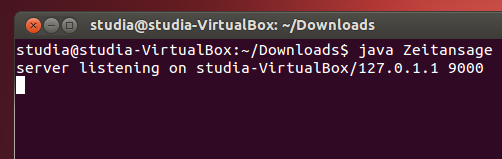
\includegraphics[width=0.4 \linewidth]{images/13}
	\caption{Gestartetes Programm Zeitanzeige}
\end{figure}

\subsection{Fazit}
Beim Ausführen des kompilierten Programms sollte darauf geachtet werden, dass man den Namen der entstandenen Datei \textbf{ohne} .class dahinter angibt. Alles in allem war diese Aufgabe leicht zu lösen und es gab keine Probleme.

\section{Aufgabe 2: b}

\subsection{Aufgabenstellung}
Das Programm kann wahlweise auch durch Angabe von Konfigurationsparametern gestartet
werden, z.B.: java Zeitansage 127.0.0.1 9099 (0,5 Punkte)

\subsection{Vorbereitung}
Bei dieser Aufgabe wird angenommen, dass die vorherige Aufgabe erledigt wurde und es eine kompilierte Version des Zeitansage Programms gibt.

\subsection{Durchführung}
Zeitansage mit Parametern aufrufen

\begin{lstlisting}
java Zeitansage 127.0.0.1 9099
\end{lstlisting}

\begin{figure}[H]
	\centering
	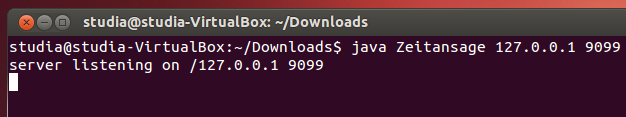
\includegraphics[width=0.4 \linewidth]{images/14}
	\caption{Zeitanzeige mit Parametern}
\end{figure}

\subsection{Fazit}
Das Ausführen des Programms mit Parametern ist ähnlich einfach wie die vorherige Aufgabenstellung. Es gab auch hier keine Probleme.

\section{Aufgabe 2: c}

\subsection{Aufgabenstellung}
Uberlegen Sie sich, wie man ermitteln kann, auf welchem Port der Service gestartet wurde! (1 Punkt)


\subsection{Vorbereitung}
Um den Port zu ermitteln muss zunächst einmal das Programm gestartet werden.

\subsection{Durchführung}
Wir benutzen für diese Aufgabe das Tool netstat.
\begin{lstlisting}
netstat -tulpn
\end{lstlisting}

\begin{figure}[H]
	\centering
	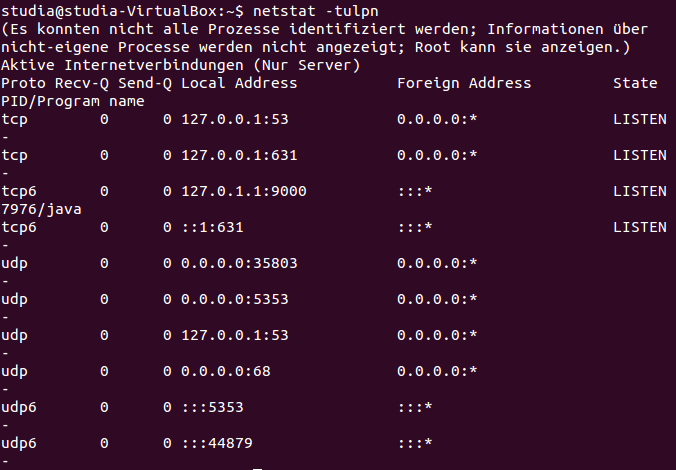
\includegraphics[width=0.4 \linewidth]{images/15}
	\caption{netstat -tulpn}
\end{figure}
In der angezeigten Liste müssen wir nur noch nach unserem Javaprogramm Ausschau halten.

\subsection{Fazit}
Mit dem Programm \texttt{netstat} kann man herausfinden welcher Prozess welchen Port verwendet. Bei dieser Aufgabe gab es keine Schwierigkeiten.

\section{Aufgabe 2: d}

\subsection{Aufgabenstellung}
Testen Sie den lokalen Server mit Hilfe der telnet-Anwendung. Sehen Sie dazu den Quellcode von Zeitanzeige.java an und verwenden Sie die dort angegebene Port-Konfiguration. (1 Punkt)

\subsection{Vorbereitung}
Ausführliche Inspektion des Quellcodes und starten des Programms \texttt{Zeitansage}.
Einlesen in die Telnet Dokumentation.

\subsection{Durchführung}
Mit gestartetem Java Programm eine Telnet-Verbindung zu \texttt{localhost} herstellen.
\begin{lstlisting}
telnet \\localhost 9000
\end{lstlisting}
\begin{figure}[H]
	\centering
	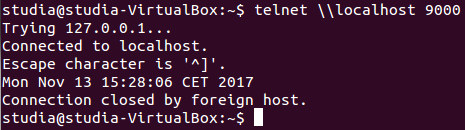
\includegraphics[width=0.4 \linewidth]{images/17}
	\caption{Telnetanfrage des Clients}
\end{figure}
\begin{figure}[H]
	\centering
	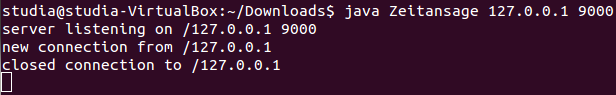
\includegraphics[width=0.4 \linewidth]{images/16}
	\caption{Ausgabe auf dem Server}
\end{figure}

\subsection{Fazit}
Bei dieser Aufgabe trat folgendes Problem auf: Wenn \texttt{Zeitansage} ohne Parameter gestartet wurde, lief es auf \texttt{127.0.1.1} und nicht auf \texttt{lokalhost} (127.0.0.1). Das konnte behoben werden indem \texttt{Zeitansage} mit den Parametern \texttt{127.0.0.1} und \texttt{9000} aufgerufen wurde.

\section{Aufgabe 2: e}

\subsection{Aufgabenstellung}
Testen Sie auch die Zeitansage Services der anderen Teilnehmer durch Zugriff auf deren Rechner. Lassen Sie dazu die IP-Adressen anderer Teilnehmer geben und stimmen Sie die verwendeten Ports ab. (1 Punkt)
Der Standard-Port für den Service ist 13. Probieren Sie diese Konfiguration; was beobachten Sie?


\subsection{Vorbereitung}
Programm \texttt{Zeianzeige} ohne Parameter starten. Anderen Client bereithalten um damit eine Telnetanfrage durchzuführen.

\subsection{Durchführung}
Auf dem anderen Client, in unserem Fall eine andere VM, die Telnetanfrage in Richtung des Servers senden.

\begin{lstlisting}
telnet 192.168.56.101 9000
\end{lstlisting}

\subsection{Fazit}
Siehe da, geht nicht :(